\documentclass[tikz, border=10pt]{standalone}
% cf http://cloford.com/resources/colours/websafe1.htm
\definecolor{sv-all}{RGB}{255,153,255}
\definecolor{sv-gxe-m2}{RGB}{255,204,255}
\definecolor{sv}{RGB}{255,153,255}
\definecolor{m1}{RGB}{153,153,255}
\definecolor{m2}{RGB}{153,255,153}
\definecolor{ge}{RGB}{255,255,153}
\definecolor{sp}{RGB}{255,153,153}
\definecolor{vi}{RGB}{255,204,153}
\definecolor{ma}{RGB}{204,255,153}
\definecolor{hedo}{RGB}{102,102,204}
\definecolor{nap}{RGB}{102,204,102}
\definecolor{ca}{RGB}{255,51,0}
\definecolor{half}{RGB}{153,153,0}

\definecolor{level-1}{RGB}{255,204,255}
\definecolor{level-2}{RGB}{153,153,255}
\definecolor{level-3}{RGB}{153,255,153}
\definecolor{level-4}{RGB}{255,255,153}
\definecolor{level-5}{RGB}{255,153,153}
\definecolor{level-6}{RGB}{255,204,153}
\definecolor{level-7}{RGB}{204,255,153}

\usetikzlibrary{
  mindmap,
  decorations.pathreplacing,    % paths with shoapes of curly braces
  positioning,     % positions like above of node
  fit              % legend bounding box fitting all nodes
}
\tikzset{
  node distance=4ex and 4ex,
  % on grid,  % node distance from the centers
  every node/.style = {
    rectangle,
    minimum width=5em,
    minimum height=3ex,
    text depth=1pt,
    draw,
    outer sep = 2pt,
    inner sep = 3pt
  },
  every edge/.style = {->,draw},
  virtual/.append style = {draw=none, circle, minimum width=1em},
  % virtual/.append style = {draw, color=black!50},   % debugging purposes
  several-all/.append style = {fill = sv-all},
  several-gxe-m2/.append style = {fill = sv-gxe-m2},
  m1/.append style = {fill = m1},
  m2/.append style = {fill = m2},
  gxe/.append style = {fill = ge},
  sp/.append style = {fill = sp},
  vi/.append style = {fill = vi},
  ma/.append style = {fill = ma},
  aux/.append style = {fill = none},
  hedo/.append style = {fill = hedo},
  nap/.append style = {fill = nap},
  ca/.append style = {fill = ca},
  half/.append style = {fill = half},
  legendkey/.append style = {minimum width=3ex},
  legendtext/.append style = {draw=none, fill = black!10},
  ->,        % arrows for all
  >=stealth  % arrow type
}
\pgfdeclarelayer{background}
\pgfsetlayers{background,main}


\begin{document}

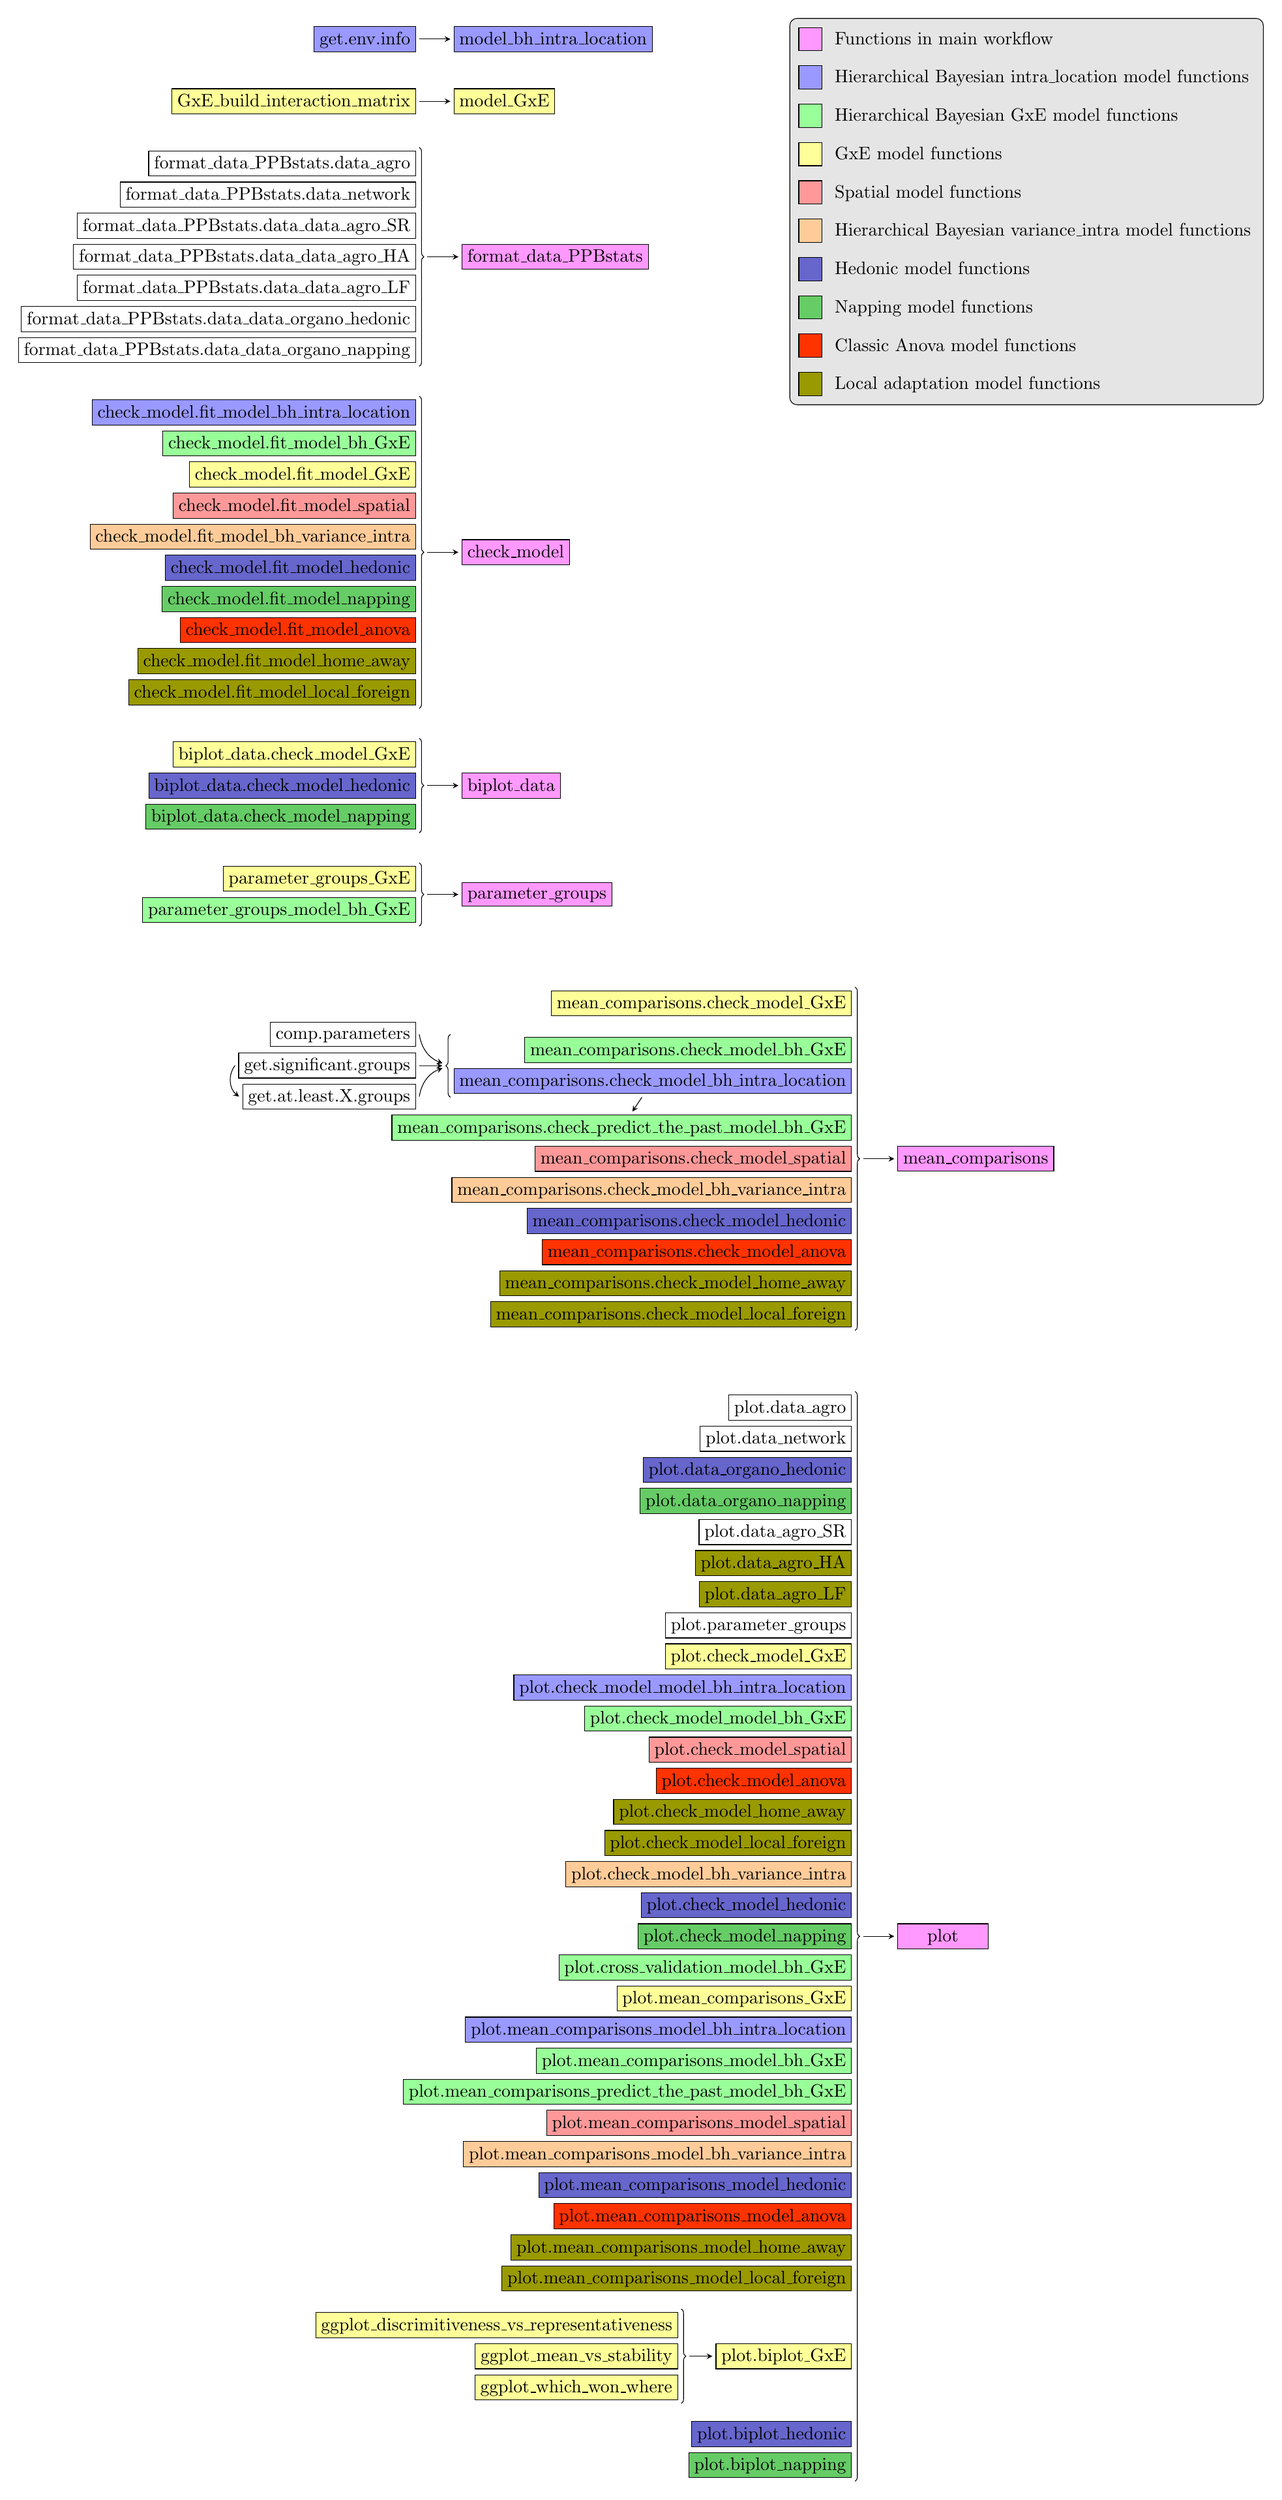
\begin{tikzpicture}

  %% Model 1
  \node [m1] (GEI) {get.env.info};
  \node [m1, right=of GEI] (m1) {model\_bh\_intra\_location};
  \draw (GEI) to (m1);


  %% GxE
  \node [gxe, below=of GEI.east, left, yshift=-4ex] (GEBIM) {GxE\_build\_interaction\_matrix};
  \node [gxe, right=of GEBIM] (GxE) {model\_GxE};
  \draw (GEBIM) to (GxE);


  %% format data
  \node [aux, below=of GEBIM.east, left, yshift=-4ex] (fda) {format\_data\_PPBstats.data\_agro};
  \node [aux, below=of fda.east, left] (fdn) {format\_data\_PPBstats.data\_network};
  \node [aux, below=of fdn.east, left] (fdasr) {format\_data\_PPBstats.data\_data\_agro\_SR};
  \node [aux, below=of fdasr.east, left] (fdahs) {format\_data\_PPBstats.data\_data\_agro\_HA};
  \node [aux, below=of fdahs.east, left] (fdalf) {format\_data\_PPBstats.data\_data\_agro\_LF};
  \node [aux, below=of fdalf.east, left] (fdoh) {format\_data\_PPBstats.data\_data\_organo\_hedonic};
  \node [aux, below=of fdoh.east, left] (fdon) {format\_data\_PPBstats.data\_data\_organo\_napping};
  
  \draw [-, decorate,decoration=brace] (fda.north east) -- (fdon.south east)
    node [midway, virtual, xshift=-4pt] (X0) {};
  \node [several-all, right=of X0] (fd) {format\_data\_PPBstats};
  \draw (X0) to (fd);
  

  %% check_model
  \node [m1, below=of fdon.east, left, yshift=-4ex] (cmm1) {check\_model.fit\_model\_bh\_intra\_location};
  \node [m2, below=of cmm1.east, left] (cmm2) {check\_model.fit\_model\_bh\_GxE};
  \node [gxe, below=of cmm2.east, left] (cmgxe) {check\_model.fit\_model\_GxE};
  \node [sp, below=of cmgxe.east, left] (cmsp) {check\_model.fit\_model\_spatial};
  \node [vi, below=of cmsp.east, left] (cmvi) {check\_model.fit\_model\_bh\_variance\_intra};
  \node [hedo, below=of cmvi.east, left] (cmh) {check\_model.fit\_model\_hedonic};
  \node [nap, below=of cmh.east, left] (cmn) {check\_model.fit\_model\_napping};
  \node [ca, below=of cmn.east, left] (cma) {check\_model.fit\_model\_anova};
  \node [half, below=of cma.east, left] (cmha) {check\_model.fit\_model\_home\_away};
  \node [half, below=of cmha.east, left] (cmlf) {check\_model.fit\_model\_local\_foreign};


  \draw [-, decorate,decoration=brace] (cmm1.north east) -- (cmlf.south east)
    node [midway, virtual, xshift=-4pt] (X1) {};
  \node [several-all, right=of X1] (cm) {check\_model};
  \draw (X1) to (cm);


  %% biplot_data
  \node [gxe, below=of cmlf.east, left, yshift=-4ex] (bdgxe) {biplot\_data.check\_model\_GxE};
  \node [hedo, below=of bdgxe.east, left] (bdh) {biplot\_data.check\_model\_hedonic};
  \node [nap, below=of bdh.east, left] (bdn) {biplot\_data.check\_model\_napping};
  
  \draw [-, decorate,decoration=brace] (bdgxe.north east) -- (bdn.south east)
    node [midway, virtual, xshift=-4pt] (X1bis) {};
  \node [several-all, right=of X1bis] (bd) {biplot\_data};
  \draw (X1bis) to (bd);


  %% parameter_groups
  \node [gxe, below=of bdn.east, left, yshift=-4ex] (pggxe) {parameter\_groups\_GxE};
  \node [m2, below=of pggxe.east, left] (pgm2) {parameter\_groups\_model\_bh\_GxE};

  \draw [-, decorate,decoration=brace] (pggxe.north east) -- (pgm2.south east)
    node [midway, virtual, xshift=-4pt] (X2) {};
  \node [several-all, right=of X2] (pg) {parameter\_groups};
  \draw (X2) to (pg);


  %% mean_comparisons

  \node [aux, below=of pgm2.east, left, yshift=-12ex] (cp) {comp.parameters};
  \node [aux, below=of cp.east, left] (gsg) {get.significant.groups};
  \node [aux, below=of gsg.east, left] (galXg) {get.at.least.X.groups};

  \node [m1, right=of galXg, yshift=2ex] (MCM1) {mean\_comparisons.check\_model\_bh\_intra\_location};
  \node [m2, above=of MCM1.east, left] (MCM2) {mean\_comparisons.check\_model\_bh\_GxE};
  \node [gxe, above=of MCM2.east, left, yshift=2ex] (MCGxE) {mean\_comparisons.check\_model\_GxE};
  \node [m2, below=of MCM1.east, left, yshift=-2ex] (MCPPM2) {mean\_comparisons.check\_predict\_the\_past\_model\_bh\_GxE};
  \node [sp, below=of MCPPM2.east, left] (MCSP) {mean\_comparisons.check\_model\_spatial};
  \node [vi, below=of MCSP.east, left] (MCVI) {mean\_comparisons.check\_model\_bh\_variance\_intra};
  \node [hedo, below=of MCVI.east, left] (MCH) {mean\_comparisons.check\_model\_hedonic};
  \node [ca, below=of MCH.east, left] (MCA) {mean\_comparisons.check\_model\_anova};
  \node [half, below=of MCA.east, left] (MCHA) {mean\_comparisons.check\_model\_home\_away};
  \node [half, below=of MCHA.east, left] (MCLF) {mean\_comparisons.check\_model\_local\_foreign};

  \node [virtual, above=of MCM1.west, yshift=-4ex, xshift=4pt] (X3) {};
  \node [virtual, above=of MCM1.west, yshift=2ex] (X3bis) {};

  \draw [bend right=45] (gsg.west) to (galXg.west);
  \draw (MCM1) to (MCPPM2);

  % braces
  \draw [-, decorate,decoration=brace] (MCM1.south west) -- (X3bis);
  \draw [bend right] (cp.east) to (X3);
  \draw (gsg) to (X3);
  \draw [bend left] (galXg.east) to (X3);


  \draw [-, decorate,decoration=brace] (MCGxE.north east) -- (MCLF.south east)
    node [midway, virtual, xshift=-4pt] (X4) {};
  \node [several-all, right=of X4] (MC) {mean\_comparisons};
  \draw (X4) to (MC);


  %% plot
  \node [, below=of MCLF.east, left, yshift=-8ex] (PDA) {plot.data\_agro};
  \node [, below=of PDA.east, left] (PDN) {plot.data\_network};
  \node [hedo, below=of PDN.east, left] (PDOH) {plot.data\_organo\_hedonic};
  \node [nap, below=of PDOH.east, left] (PDOA) {plot.data\_organo\_napping};
  \node [aux, below=of PDOA.east, left] (PDASR) {plot.data\_agro\_SR};
  \node [half, below=of PDASR.east, left] (PDAHA) {plot.data\_agro\_HA};
  \node [half, below=of PDAHA.east, left] (PDALF) {plot.data\_agro\_LF};
  
  \node [aux, below=of PDALF.east, left] (GPG) {plot.parameter\_groups};
  
  \node [gxe, below=of GPG.east, left] (GCMGxE) {plot.check\_model\_GxE};
  \node [m1, below=of GCMGxE.east, left] (GCMM1) {plot.check\_model\_model\_bh\_intra\_location};
  \node [m2, below=of GCMM1.east, left] (GCMM2) {plot.check\_model\_model\_bh\_GxE};
  \node [sp, below=of GCMM2.east, left] (GCMSP) {plot.check\_model\_spatial};
  \node [ca, below=of GCMSP.east, left] (GCMA) {plot.check\_model\_anova};
  \node [half, below=of GCMA.east, left] (GCMHA) {plot.check\_model\_home\_away};
  \node [half, below=of GCMHA.east, left] (GCMLF) {plot.check\_model\_local\_foreign};
  \node [vi, below=of GCMLF.east, left] (GCMVI) {plot.check\_model\_bh\_variance\_intra};
  \node [hedo, below=of GCMVI.east, left] (GCMH) {plot.check\_model\_hedonic};
  \node [nap, below=of GCMH.east, left] (GCMN) {plot.check\_model\_napping};

  \node [m2, below=of GCMN.east, left] (GCVM2) {plot.cross\_validation\_model\_bh\_GxE};

  \node [gxe, below=of GCVM2.east, left] (GMCGxE) {plot.mean\_comparisons\_GxE};
  \node [m1, below=of GMCGxE.east, left] (GMCM1) {plot.mean\_comparisons\_model\_bh\_intra\_location};
  \node [m2, below=of GMCM1.east, left] (GMCM2) {plot.mean\_comparisons\_model\_bh\_GxE};
  \node [m2, below=of GMCM2.east, left] (GMCPPM2) {plot.mean\_comparisons\_predict\_the\_past\_model\_bh\_GxE};
  \node [sp, below=of GMCPPM2.east, left] (GMCSP) {plot.mean\_comparisons\_model\_spatial};
  \node [vi, below=of GMCSP.east, left] (GMCVI) {plot.mean\_comparisons\_model\_bh\_variance\_intra};
  \node [hedo, below=of GMCVI.east, left] (GMCH) {plot.mean\_comparisons\_model\_hedonic};
  \node [ca, below=of GMCH.east, left] (GMCA) {plot.mean\_comparisons\_model\_anova};
  \node [half, below=of GMCA.east, left] (GMCHA) {plot.mean\_comparisons\_model\_home\_away};
  \node [half, below=of GMCHA.east, left] (GMCLF) {plot.mean\_comparisons\_model\_local\_foreign};
  \node [gxe, below=of GMCLF.east, left, yshift=-6ex] (GBGxE) {plot.biplot\_GxE};
  \node [gxe, left=of GBGxE] (GMS) {ggplot\_mean\_vs\_stability};
  \node [gxe, above=of GMS.east, left] (GDR) {ggplot\_discrimitiveness\_vs\_representativeness};
  \node [gxe, below=of GMS.east, left] (GWWW) {ggplot\_which\_won\_where};
  \draw [-, decorate,decoration=brace] (GDR.north east) -- (GWWW.south east)
  node [midway, virtual, xshift=-4pt] (X5) {};
  \draw (X5) to (GBGxE);
  
  \node [hedo, below=of GBGxE.east, left, yshift=-6ex] (PBH) {plot.biplot\_hedonic};
  \node [nap, below=of PBH.east, left] (PBN) {plot.biplot\_napping};

  \draw [-, decorate,decoration=brace] (PDA.north east) -- (PBN.south east)
  node [midway, virtual, xshift=-4pt] (X6) {};
  \node [several-all, right=of X6] (P) {plot};
  \draw (X6) to (P);

  %% legend
  \node[several-all,legendkey]  (LS)  [right=of m1, xshift=6em] {};
  \node[right,legendtext] (LStext) at (LS.east) {Functions in main workflow};

  \node[m1,legendkey]  (LM1)  [below=of LS,yshift=3ex] {};
  \node[right,legendtext] (LM1text) at (LM1.east) {Hierarchical Bayesian intra\_location model functions};

  \node[m2,legendkey]  (LM2)  [below=of LM1,yshift=3ex] {};
  \node[right,legendtext] at (LM2.east) {Hierarchical Bayesian GxE model functions};

  \node[gxe,legendkey]  (LGxE)  [below=of LM2,yshift=3ex] {};
  \node[right,legendtext] at (LGxE.east) {GxE model functions};

  \node[sp,legendkey]  (LSP)  [below=of LGxE,yshift=3ex] {};
  \node[right,legendtext] at (LSP.east) {Spatial model functions};

  \node[vi,legendkey]  (LVI)  [below=of LSP,yshift=3ex] {};
  \node[right,legendtext] at (LVI.east) {Hierarchical Bayesian variance\_intra model functions};

  \node[hedo,legendkey]  (LH)  [below=of LVI,yshift=3ex] {};
  \node[right,legendtext] at (LH.east) {Hedonic model functions};

  \node[nap,legendkey]  (LN)  [below=of LH,yshift=3ex] {};
  \node[right,legendtext] at (LN.east) {Napping model functions};

  \node[ca,legendkey]  (LCA)  [below=of LN,yshift=3ex] {};
  \node[right,legendtext] at (LCA.east) {Classic Anova model functions};

  \node[half,legendkey]  (LHALF)  [below=of LCA,yshift=3ex] {};
  \node[right,legendtext] at (LHALF.east) {Local adaptation model functions};

  %% legend bounding box
  \begin{pgfonlayer}{background}
    \node[
      fill=black!10,
      rounded corners,
      fit = (LS) (LHALF) (LM1text)
    ] {};
  \end{pgfonlayer}

\end{tikzpicture}

\end{document}
